% figs_malhas_comparacao.tex: figuras de malhas da comparacao entre malhas fixas e refinamento pela banda.
% Gerado por figuras_malhas.py (python3 figuras_malhas.py comparacao); usa malhas.py.

\begin{figure}[htbp]
  \centering
  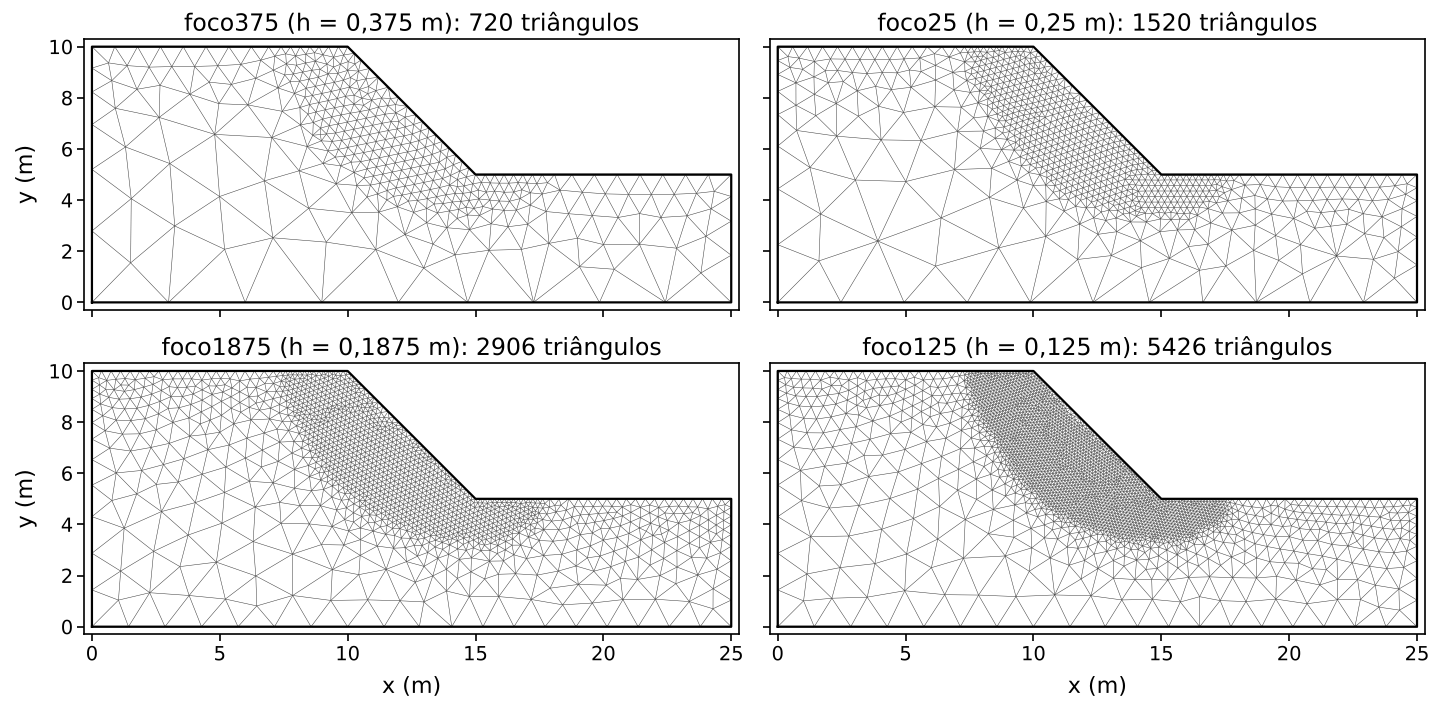
\includegraphics[width=\textwidth]{figuras/ref_malhas_fixas.png}
  \caption{Malhas fixas focadas da comparação (triângulos lineares, gmsh): tamanho $h$ de
    0,375, 0,25, 0,1875 e 0,125~m numa faixa de 0,75~m em torno das bandas de ruptura
    ($\sqrt{J_2} \geq 0{,}1$ do máximo) do caso determinístico e das realizações 0 a 31 de um
    estudo anterior na malha original; fora dela, 0,9~m perto da superfície e até 3~m no interior.
    Talude de Vargas Ceron et al.\ (2025), Seção~6: $H = 5$~m, $\beta = 45^\circ$, pé em (15, 5)
    e crista em (10, 10). A foco125 é a referência das diferenças relativas.}
  \label{fig:ref:malhas_fixas}
\end{figure}

\begin{figure}[htbp]
  \centering
  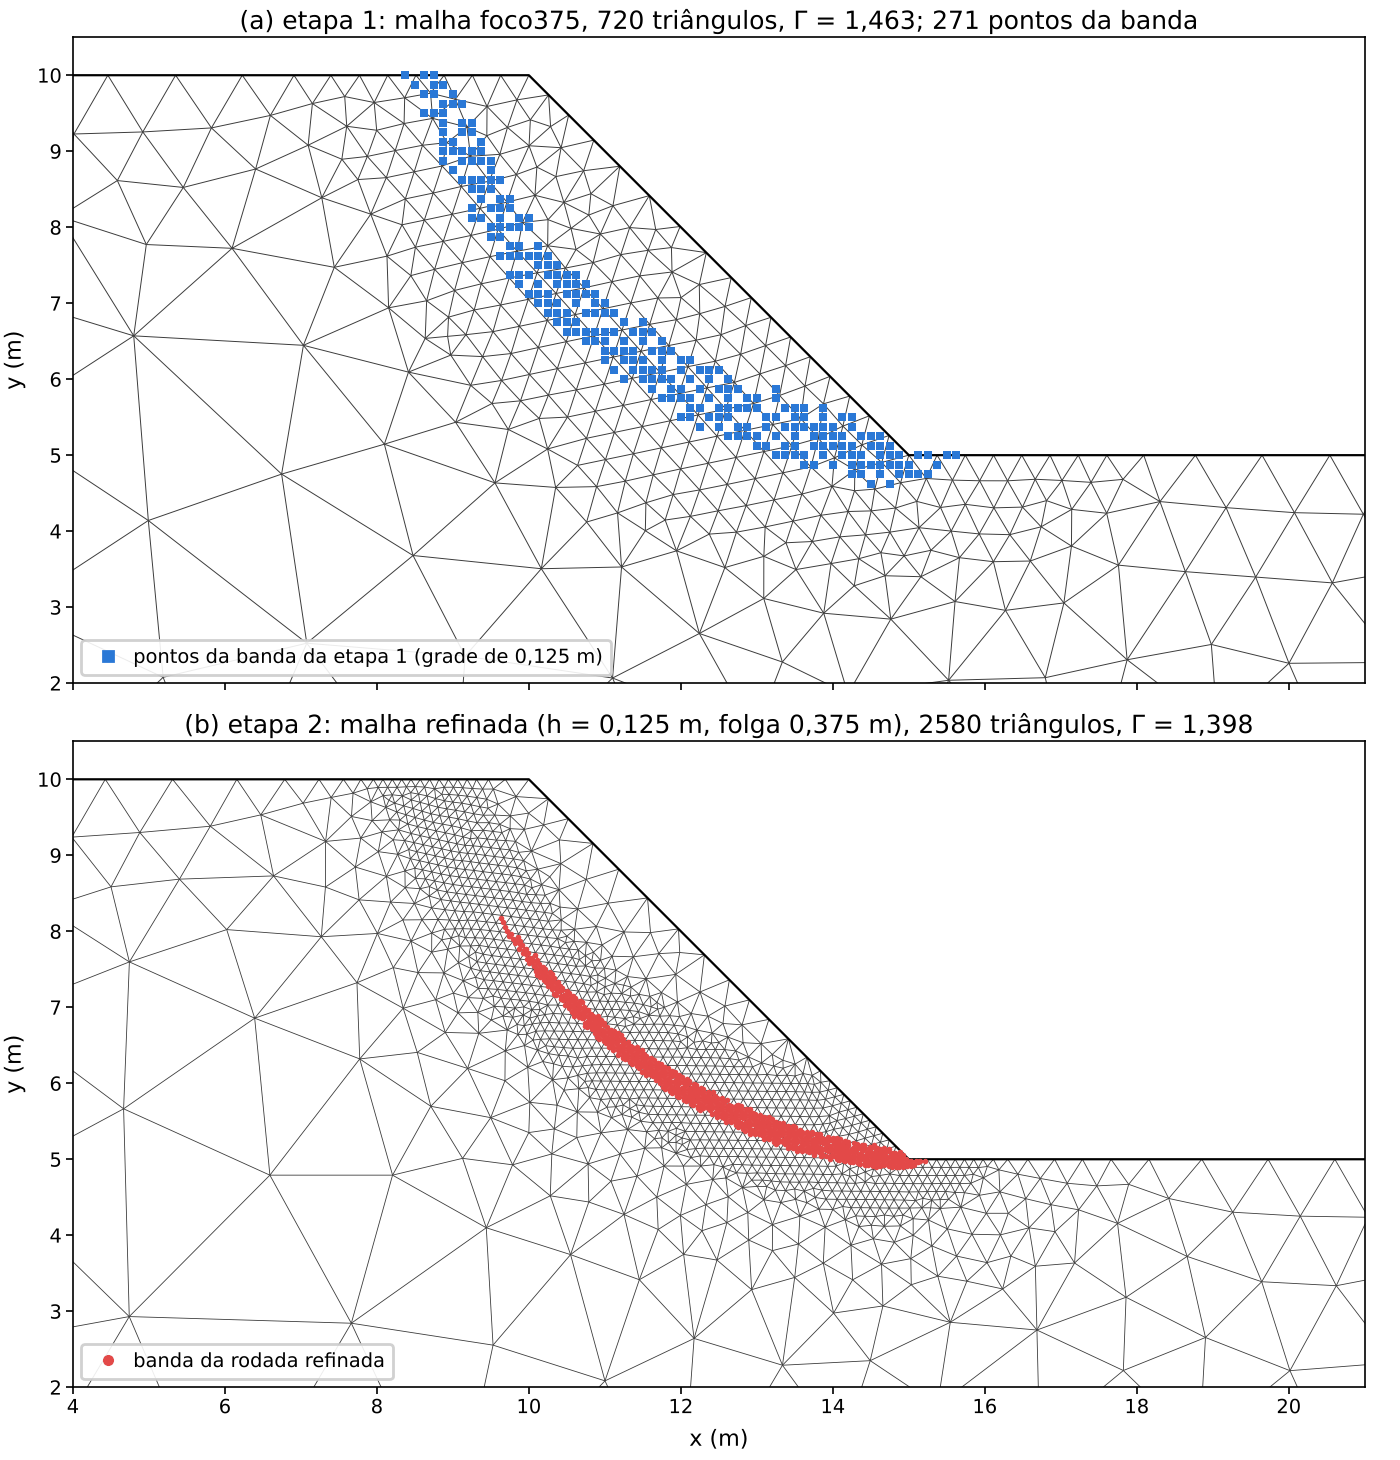
\includegraphics[width=\textwidth]{figuras/ref_metodo_det.png}
  \caption{Refinamento pela banda no caso determinístico (ampliação da região do talude).
    (a) Etapa~1: rodada na malha foco375 (720 triângulos, $\Gamma = 1{,}463$); os 271 pontos
    azuis são os pontos de integração da banda dessa rodada ($\sqrt{J_2}$ da deformação plástica
    $\geq 0{,}1$ do máximo no instante do fator, isto é, no $t_h$ do menor FS) arredondados numa
    grade de 0,125~m, que o \texttt{refina\_banda.py} acrescenta ao \texttt{.geo}.
    (b) Etapa~2: malha refinada com $h = 0{,}125$~m até 0,375~m desses pontos (2580 triângulos,
    contra 5426 da foco125) e, em vermelho, a banda da rodada refinada, com a mesma definição
    ($\Gamma = 1{,}398$).}
  \label{fig:ref:metodo_det}
\end{figure}

\begin{figure}[htbp]
  \centering
  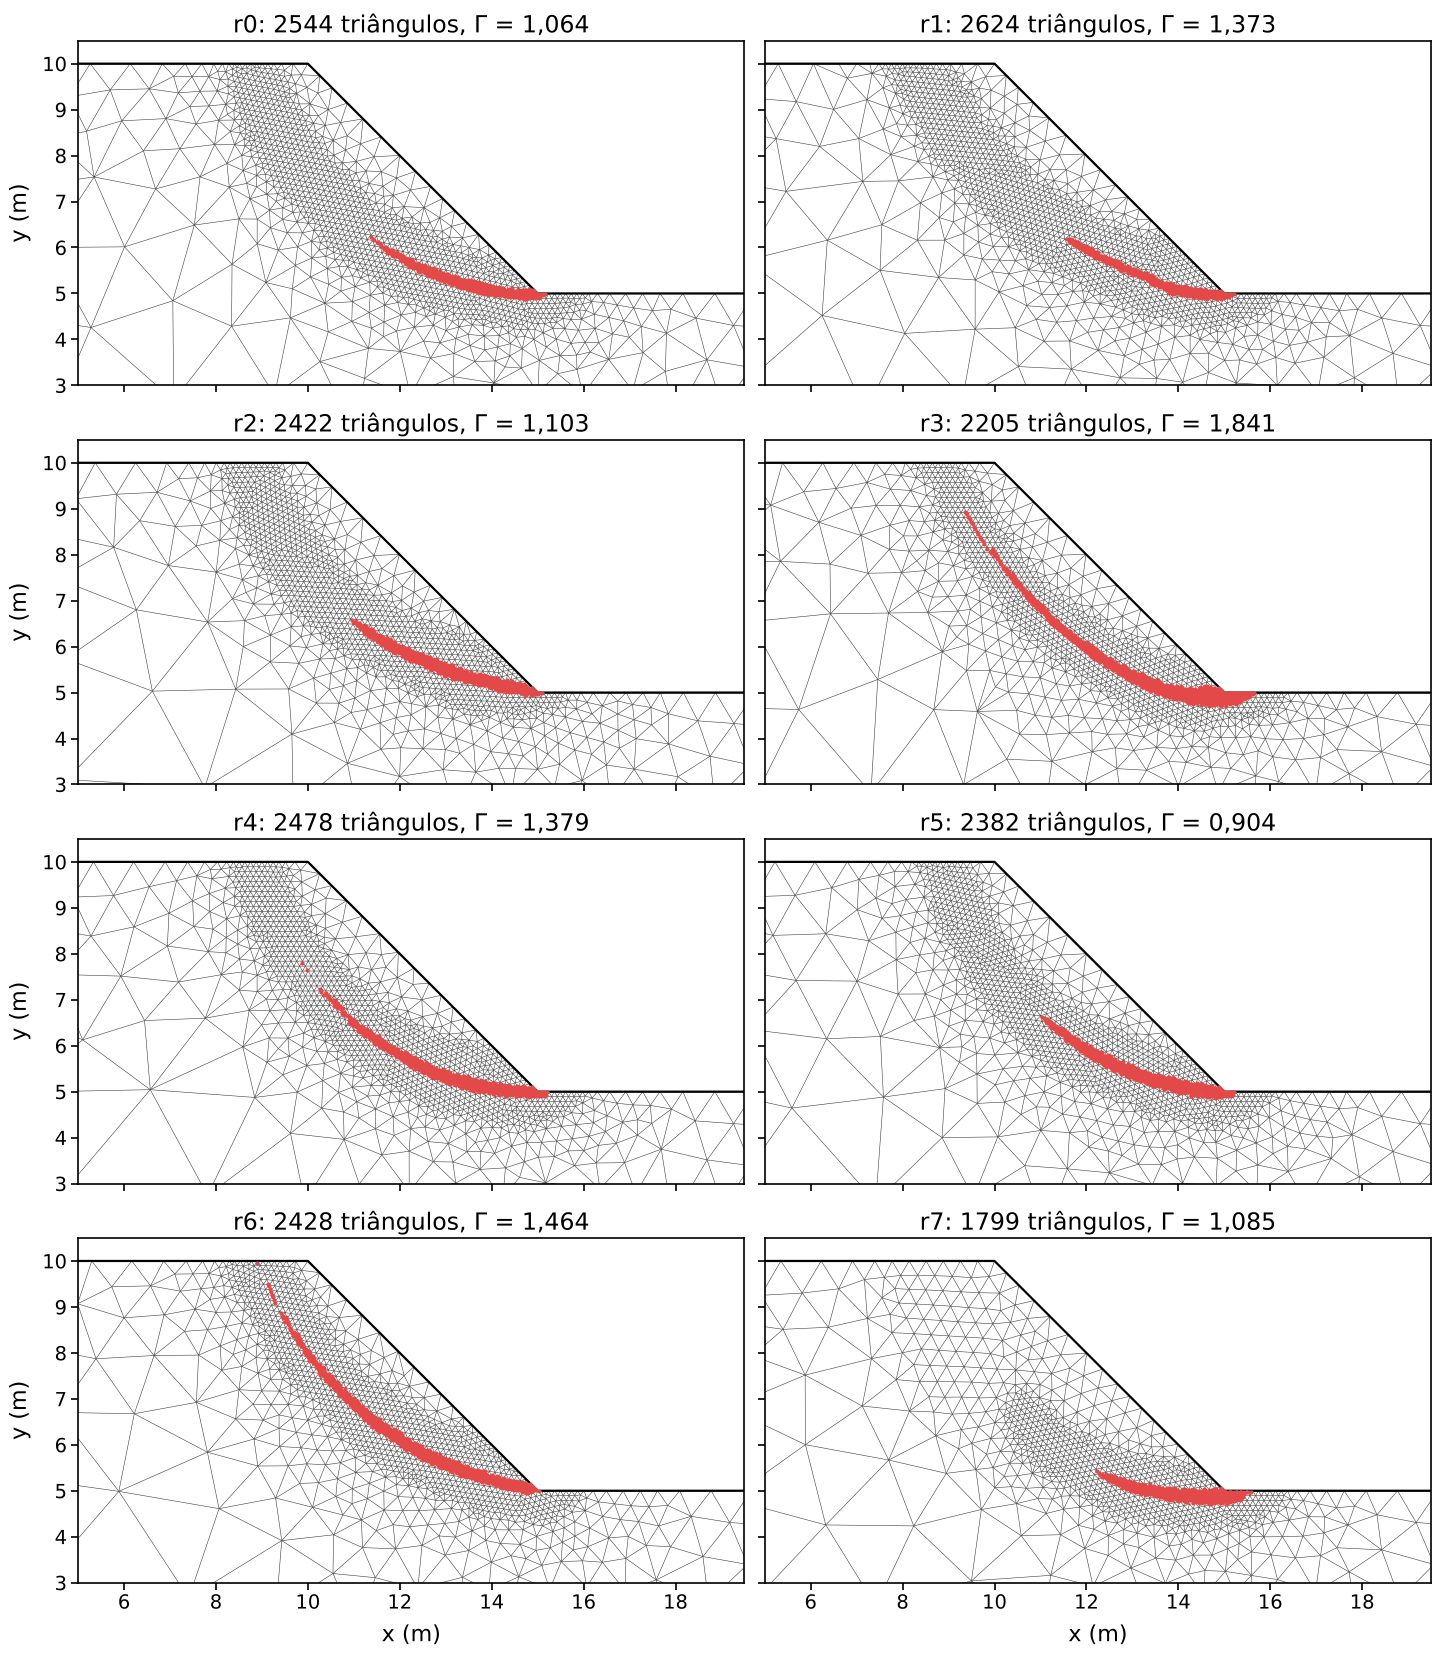
\includegraphics[width=\textwidth]{figuras/ref_refinadas.png}
  \caption{Malhas refinadas (etapa~2 a partir da foco375: $h = 0{,}125$~m até 0,375~m da banda da
    etapa~1) das realizações r0 a r7, com a banda de ruptura de cada rodada refinada (em vermelho:
    pontos de integração com $\sqrt{J_2}$ da deformação plástica $\geq 0{,}1$ do máximo no instante
    do fator) e o fator $\Gamma$ obtido. O número de triângulos acompanha a extensão da banda da
    etapa~1: de 1799 (r7, banda curta junto ao pé) a 2624 (r1), contra 5426 da malha fixa foco125.}
  \label{fig:ref:refinadas}
\end{figure}
